\section{More about Event-B}

\subsection{Decomposition and Composition}

Decomposition and composition are two related approaches, that we use to partition a system, to allow us to work on smaller, manageable sub-models. Figure~\ref{fig:decomp2} illustrates the shared-event decomposition approach~\cite{decomp2010c} which we make use of in our code generation approach. An alternative shared-variable approach is described in~\cite{AbrialH07}. \emph{v1} and \emph{v2} are disjoint sets of variables, and \emph{p} and \emph{q} are disjoint sets of parameters. \emph{g} and \emph{a} are guards and actions that range over the  variables and parameters. In the shared-event decomposition approach the system is partitioned so that each variable is allocated to a single machine. In Fig.~\ref{fig:decomp2}, the variables of machine $m$ are partitioned into the sets $v1$ and $v2$ and decomposed into $m_a$ and $m_b$ respectively. The decomposed events have guards and actions which involve their respective variable partitions. The composed machine construct contains references to the decomposed machines. It keeps track of the refinement relationship between the abstract machine and the decomposed machines. In the decomposition, it is the synchronization of events, in different decomposed machines, that refines a single abstract event. 

The main purpose of using this form of event decomposition is that it reduces the size of the models, therefore making modelling and proof easier. The decomposed machines can be refined without restriction. For code generation, the synchronization of events provides a suitable basis for modelling procedures and procedure calls.
 %
\begin{figure}
\centering
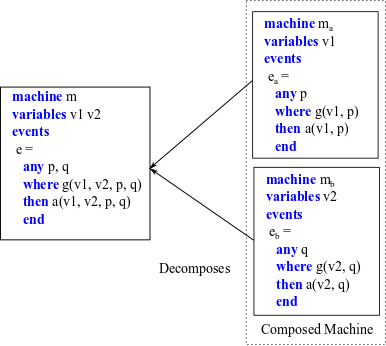
\includegraphics[width=0.5\textwidth]{graphics/Decomp2.png}
\caption{Decomposition}
\label{fig:decomp2}
\end{figure}
%
\subsection{Theories}
The theory plug-in provides a mechanism for extending the Event-B proof capabilities, and addition of new mathematical types~\cite{issam2013}. Proof obligations will be generated to verify the soundness of the augmented prover. We can make use of the following sections in the theory plug-in.

\begin{enumerate}
\item Type Parameters: A theory can define type parameters to be used as polymorphic types.
\item Datatypes: Used to define simple data types, which can be added using a type constructor and element constuctors.
\item Operators: The operators section can be used to define polymorphic operators, such as the sequence described as an ordered list~\cite{issam2013}. 
\item Axiomatic Definitions: These are defined to produce types, when no suitable type constructors or datatypes can be used as a basis for construction.
\item Theorems: Polymorphic theorems can be used to assist with the proof of newly introduced definitions. 
\item Rewrite rules: Rewrite rules define how to rewrite formulas to equivalent forms. When a rewrite rule is defined, the author specifies whether the rule should be applied automatically, or during an interactive proof session.
\item Inference rules: Rules are matched against sequent goals. If a match is found, a backward proof step is performed. The rule may also match a hypotheses of a sequent, where a forward proof step is performed.
\end{enumerate}
\subsection{ProB}
